\section{Industrial Context}

\subsection{The fuel element of pressurized water reactor}

The industrial French nuclear fleet is made of Pressurized Water Reactor
(PWR), as well as three quarters of power reactors worldwide.

A fuel element is a stack of fuel pellets enclosed in a cladding made of
an alloy of Zirconium. This fuel element is thus called a fuel rod. A
fuel rod is almost 4 meters long, and the cladding outer diameter is
$9.5$mm wide.

% ![Typical dimensions of a fuel pellet](img/FuelPellet.pdf ""){#fig:hho:fuel_pellet width=75%}

\begin{figure}[H]
  \centering
  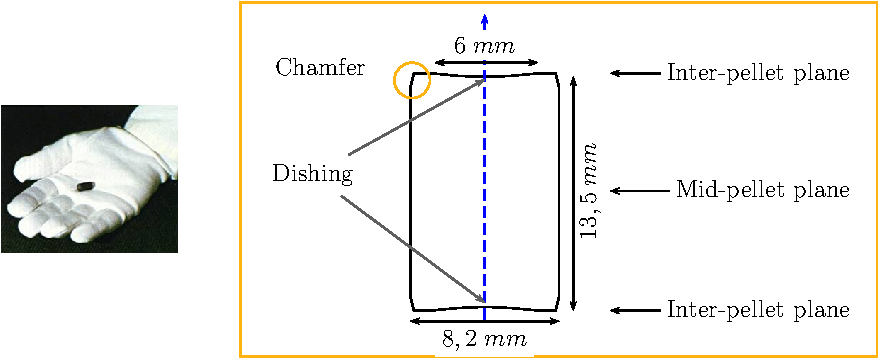
\includegraphics[width=10.cm]{../chapter_000_introduction/figures/FuelPellet.pdf}
  \caption{Typical dimensions of a fuel pellet}
  \label{fig:hho:fuel_pellet}
\end{figure}

The fuel pellet itself is mostly made of Uranium dioxide \(UO_{2}\) or a
Mixed Oxide (MOX) which also incorporates Plutonium. The typical
dimensions of a fuel pellet are reported on Figure \ref{fig:hho:fuel_pellet}.
The main nuclear reaction in the fuel is the fission of dioxide
\(\mbox{}^{235}U\) isotope of Uranium and in several isotopes
of Plutonium. The presence of dishings have significant influence on the
behaviour of the pellet in power transient, as discussed in Section
\ref{sec:hho:off_normal_operating_conditions}.

Fuels rod are gathered in an assembly which typically holds \(264\) fuel
rods. In a \(900\,MWe\) PWR, the core contains \(157\) assemblies for a
total of approximatively \(41\,000\) fuels rods.

In the reactor core, the fuel rod is surrounded by pressurized water (at
around \(15,5\, MPa\) and a temperature of about $320$°C). The role of the
pressurized water is twofold:

\begin{itemize}
    \item Thermalizing neutrons, i.e. absorbing part of a neutron energy down to
    a level for which the cross-section of \(\mbox{}^{235}U\) is
    significantly higher \footnote{Fission cross section of \(\mbox{}^{235}U\) for slow thermal
    neutrons is about \(584\) barns which is significantly higher that the
    cross-section of fast neutrons which is typically on the order of 1
    barn.}.
    \item Extracting the heat generated by those reactions. Hence, the water in
    the reactor core is generally denoted as the coolant.
\end{itemize}

% \footnotetext[U235]{Fission cross section \(\mbox{}^{235}U\) of for slow thermal
% neutrons is about \(584\) barns which is significantly higher that the
% cross-section of fast neutrons which is typically on the order of 1
% barn.}

% - Thermalizing neutrons, i.e. absorbing part of a neutron energy down to
%   a level for which the cross-section of \(\mbox{}^{235}U\) is
%   significantly higher[^U235].
% - Extracting the heat generated by those reactions. Hence, the water in
%   the reactor core is generally denoted as the coolant.

% [^U235]: Fission cross section \(\mbox{}^{235}U\) of for slow thermal
% neutrons is about \(584\) barns which is significantly higher that the
% cross-section of fast neutrons which is typically on the order of 1
% barn.

From a safety point of view, the integrity of the cladding, i.e. its
ability to retain the fuel from disseminating radioactive elements in
the coolant, must be assessed.

This point is studied by the experimental campaigns in research reactors
and the development of simulation tools worldwide
\cite{garcia_mono-dimensional_2002, williamson_multidimensional_2012, di_marcello_transuranus_2014, largenton_cyrano3_2014, petry_cyrano3_2015, qi_qualification_2019,scolaro_offbeat_2020}.

In particular, CEA develops a numerical platform called \texttt{PLEIADES}
\cite{marelle_new_2016} to simulate the behaviour of nuclear fuel elements
for various nuclear systems (PWR, Sodium Fast Reactor, Material Testing Reactor) in normal and
off-normal operating conditions and also experimental devices
\cite{lainet_recent_2013, helfer_licos_2015}. In this platform, the
\texttt{ALCYONE} fuel performance code is dedicated to PWR fuels
\cite{helfer_recent_2015, marelle_new_2016, guenot-delahaie_simulation_2017}.

The precise understanding of the evolution of the fuel rod under
irradiation is made all the more difficult due to the numerous coupled
physical phenomena at play \cite{JRC83478}. The next section is
devoted to an overview of the fuel rod evolution under irradiation in
normal and off-normal operating conditions.

\subsection{A compendium of the fuel rod evolution under irradiation}

A complete description of fuel rod evolution under irradiation is out of
the scope of this document. The interested reader may refer to the
reference books on that matter for further details
\cite{bailly_nuclear_1999, cea_nuclear_2009}. This paragraph only presents
the most relevant phenomena occurring in the fuel rod in the perspective
of our work.

\paragraph{Normal operating conditions}
\label{sec:hho:normal_operating_conditions}

Nuclear reactions in the fuel lead to an important temperature gradient
in the fuel pellet. For a nominal power of about \(200\,W.cm^{-1}\),
this radial gradient is typically greater than \(100\,K.mm^{-1}\). This
temperature gradient induces a high level of stresses by
thermoelasticity:

\begin{itemize}
    \item The center, which is around \(1\,400\, K\), of the pellet is in
    compression.
    \item The periphery of the pellet, which is around \(1\,000\,K\), is in
    tension.
\end{itemize}

% ![Simplified classification of the observed cracks (left). Initial
% fragmentation of the fuel pellet simulated using a phase field approach
% \cite{2019_LU_HELFER_BARY_FANDEUR_UnSchemaNumeriqueEfficacePourLeTraitementDeLaFissurationFragileDesMateriauxQuasiFragilesParChampDePhase} (right). Because of a coarse mesh, this
% simulation is not totally representative of the fracture properties of
% \(UO_{2}\), i.e. the characteristic length used in the simulation, which
% must be greater than the mesh size, is too high (See Section
% @sec:phase_field:crack_nucleation). However, these simulations capture
% qualitatively the experimental crack patterns.](img/CrackNetwork.pdf ""){#fig:hho:crack_network with=75%}

\begin{figure}[H]
  \centering
  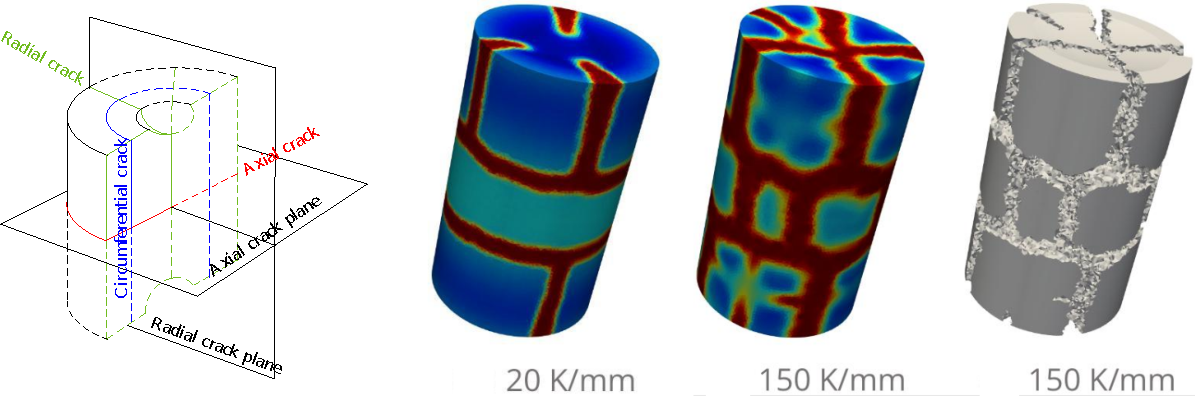
\includegraphics[width=10.cm]{../chapter_000_introduction/figures/CrackNetwork.pdf}
  \caption{Simplified classification of the observed cracks (left). Initial
  fragmentation of the fuel pellet simulated using a phase field approach
  \cite{2019_LU_HELFER_BARY_FANDEUR_UnSchemaNumeriqueEfficacePourLeTraitementDeLaFissurationFragileDesMateriauxQuasiFragilesParChampDePhase} (right). Because of a coarse mesh, this
  simulation is not totally representative of the fracture properties of
  \(UO_{2}\), i.e. the characteristic length used in the simulation, which
  must be greater than the mesh size, is too high (See Section
  \ref{sec:phase_field:crack_nucleation}). However, these simulations capture
  qualitatively the experimental crack patterns}
  \label{fig:hho:crack_network}
\end{figure}

The induced stresses far exceeds the fracture strength of Uranium
dioxide. Due to the brittle nature of Uranium dioxide, a complex cracks
network propagates in the pellet. A simple thermoelastic computation
shows that the fracture stress is reached during the reactor start-up
\cite{helfer_etude_2006}. A schematic representation of the cracked pellet,
using conventions of Figure \ref{fig:hho:crack_network} is currently used in
most \(3D\) simulations performed with the \texttt{Alcyone} fuel performance
code and can be built by inserting an axial crack in the mid-pellet
plane and \(6\) to \(8\) radial cracks, such that the fuel pellet is
divided into \(12\) to \(16\) macroscopic fragments. Most simulations
only consider half a fragment of pellet due to symmetry conditions
\cite{michel_pellet_2005}.

Numerically, initial fragmentation of the pellet has been studied in
\cite{helfer_modelisation_2017} and later by Lu et al. \cite{2019_LU_HELFER_BARY_FANDEUR_UnSchemaNumeriqueEfficacePourLeTraitementDeLaFissurationFragileDesMateriauxQuasiFragilesParChampDePhase} by a
phase field approach as depicted in Figure
\ref{fig:hho:crack_network}.

\begin{figure}[H]
  \centering
  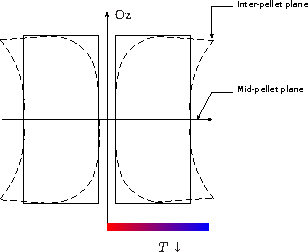
\includegraphics[width=10.cm]{../chapter_000_introduction/figures/HourGlassEffect.pdf}
  \caption{Hourglass shape of the pellet. Initial shape is depicted using solid
  lines while the hourglass shape is depicted using dashed
  lines}
  \label{fig:hho:hourglass}
\end{figure}

% ![Hourglass shape of the pellet. Initial shape is depicted using solid
% lines while the hourglass shape is depicted using dashed
% lines.](img/HourGlassEffect.pdf){#fig:hho:hourglass width=50%}

The temperature gradient in the fragments leads to the hourglassing of
the pellet, i.e. the radial displacement of points of the outer surface
of the pellet is much greater in the inter-pellet plane than in the
mid-pellet plane (see Figure \ref{fig:hho:hourglass}). After fragmentation,
the remaining stresses in the fuel are relieved by irradiation creep.

The cladding is submitted to the pressure of the coolant which far
exceeds the initial pressure in the fuel rod. The cladding, whose
temperature is between \(560\,K\) and \(600\,K\), is in compression.
Viscoplasticity, accelerated under irradiation, leads to a reduction of
the radius of the cladding.

During the first and second operating cycles, the gap between the fuel
pellet and the cladding remains open but diminishes due to three
phenomena of equal importance:

\begin{itemize}
  \item The thermal expansion of the pellet.
  \item The hourglassing of the pellet.
  \item The viscoplastic flow in the cladding due to the coolant pressure.
\end{itemize}

During the first cycle, the initial porosity of the pellet diminishes due to the
in-pile densification leading to a decrease of the fuel pellet radius
which is compensated by swelling due to solid fission products.

After the first two cycles, the gap between the fuel pellet and the
cladding is closed and a weak interaction between the pellet and the
cladding occurs. Due to the hour-glass shape of the fuel pellet, this
interaction happens earlier in the inter-pellet plane. Due to the coolant
pressure, the pellet hourglassing diminishes, a phenomena also called
fragments' repositioning. Although the contact between the pellet and
the cladding is ultimately established on the whole outer surface of the
pellet, the earlier interaction in the inter-pellet plane is visible on
the cladding on which ridges appears. After irradiation, the cladding
thus has a "bamboo"-like shape.

After a few cycles, the cladding diameter increases due to fuel-pellet
swelling. The coolant pressure is gradually compensated by the inner
pressure increase in the fuel rod due to the release of gaseous fission
products. A high burn-up (micro-)structure develops at the periphery of
the pellet. This phenomenon is called the "rim"-effect. The high burn-up
structure affects various aspect of the fuel behaviour, including
viscoplasticity and swelling.

Many advanced models describe the behaviour of fission products and
microstructural evolutions of the fuel \cite{pizzocri_sciantix_2020}. In
particular, CEA has developed the \texttt{CARACAS} \cite{boulore_approach_2017}
and \texttt{MARGARET} models \cite{noirot_margaret_2011}.

For the purpose of this document, it shall be highlighted that all those
models take into account the macroscropic mechanical state of the pellet
through the hydrostatic pressure.

\paragraph{An example of off-normal operating conditions}
\label{sec:hho:off_normal_operating_conditions}

This paragraph is devoted to the description of a less severe off-normal
operating condition, namely power transient of class II. During this
class of transient, the power generated by the fuel rod may exceed
\(450\,W.cm^{-1}\) during a few hours. A typical evolution of the
maximum temperature in the fuel pellet is reported in Figure
\ref{fig:hho:transient_power}.

Several scenarii aimed at anticipating the consequences of off-normal
operating conditions are studied experimentally and numerically:

\begin{itemize}
  \item Reactivity Initiated Accident (RIA) describes the effect of an
  unwanted fast increase in fission rate and reactor power, due for
  example to the ejection of a control rod. Such situations can notably
  be reproduced experimentally in the Cabri research reactor located at
  CEA center of Cadarache where an experimental rod can be submitted to
  a power pulse of a few micro-seconds. Simulations of such pulses using
  the \texttt{Alcyone} fuel performance code are described in
  \cite{guenot-delahaie_simulation_2017}.
  \item Loss of coolant accidents (LOCAs) describe the consequence of a
  breach in the coolant circuit in which the cladding may not be cooled
  for a few minutes. Although the nuclear reaction may rapidly stop, the
  residual power generated by the fuel rod may lead to a significant
  increase of the cladding temperature. Such situations may notably be
  studied in the Halden research reactor. Simulations of such transients
  using the \texttt{Alcyone} fuel performance code are provided by
  \cite{struzik_simulation_2017}.
\end{itemize}

% ![Evolution of the maximim temperature during a power transient of class II in a research reactor](img/TransientPowerClassII.png){#fig:hho:transient_power width=75%}

\begin{figure}[H]
  \centering
  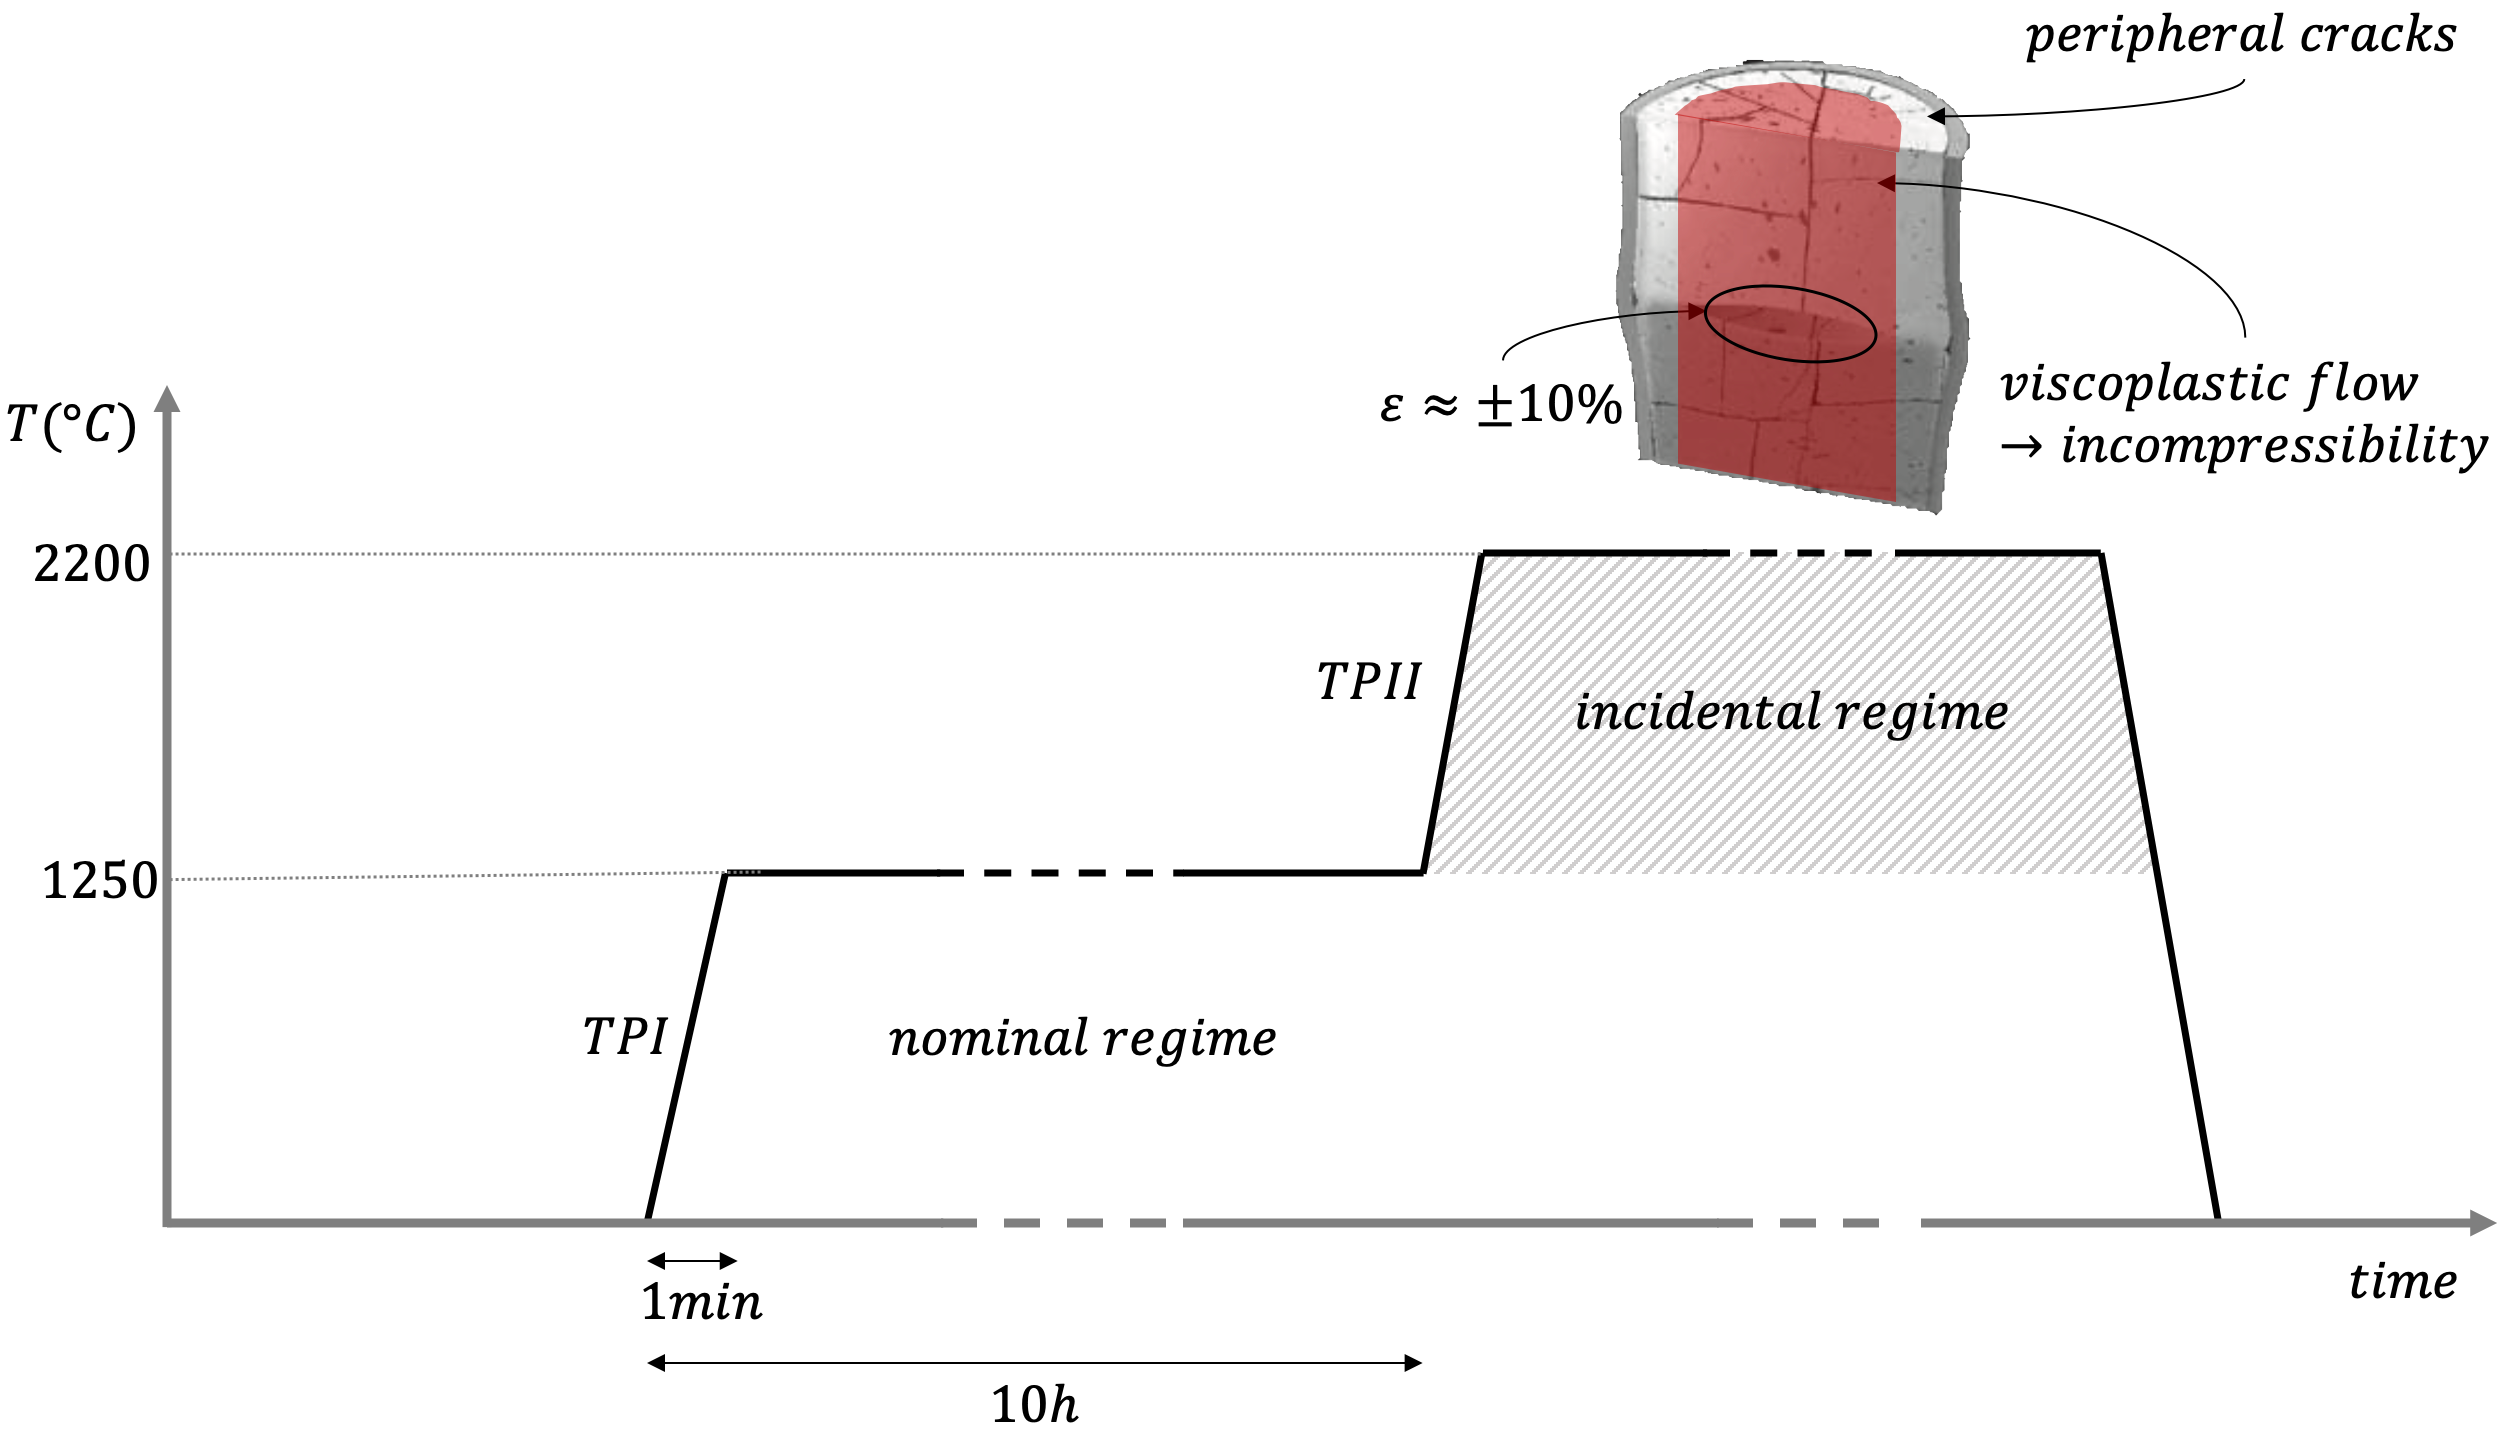
\includegraphics[width=10.cm]{../chapter_000_introduction/figures/TransientPowerClassII.png}
  \caption{Evolution of the maximim temperature during a power transient of class II in a research reactor}
  \label{fig:hho:transient_power}
\end{figure}

Swelling due to fission gas release induces an increase of cladding
radius which can lead to its failure.

% ![Typical crack network in the fuel pellet after irradiation in a research reactor](img/CrackNetwork2.pdf){#fig:hho:crack_network_2 width=75%}

\begin{figure}[H]
  \centering
  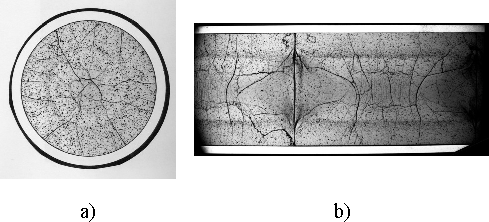
\includegraphics[width=10.cm]{../chapter_000_introduction/figures/CrackNetwork2.pdf}
  \caption{Typical crack network in the fuel pellet after irradiation in a research reactor}
  \label{fig:hho:crack_network_2}
\end{figure}

Figure \ref{fig:hho:crack_network_2} describes the typical metallographies of
a pellet after the power transient. While the primary crack network that
led to the pellet fragmentation is still visible, a secondary crack
network in the pellet appears. This secondary crack network may have a
significant and beneficial impact of the pellet-cladding interaction
during the power transient \cite{michel_3d_2008}.

Due to the viscoplasticity of the fuel at high temperature, an axial
movement of matter fills the dishings, leading to locally high strain
level. This viscoplastic behaviour of the core of the pellet also
significantly decreases the loading on the cladding.

Viscoplasticity at high temperature of uranimum dioxide, mostly
on unirradiated material, has been the subject of many studies,
including
\cite{colin_etude_2003,monerie_overall_2006, salvo_experimental_2015, salvo_experimental_2015-1, garcia_effect_2020}.

Simulations of such power transients with \texttt{Alcyone} are described in
\cite{helfer_etude_2006, michel_3d_2008}.

\subsection{Fuel behaviour at the microstructural scale}

% ![Description of the failure of a representative element volume due to
% the bubble pressurisation in the high burn-up structure
% \cite{esnoul_etude_2018}.](img/VEREsnoul.png){#fig:hho:esnoul width=75%}

\begin{figure}[H]
  \centering
  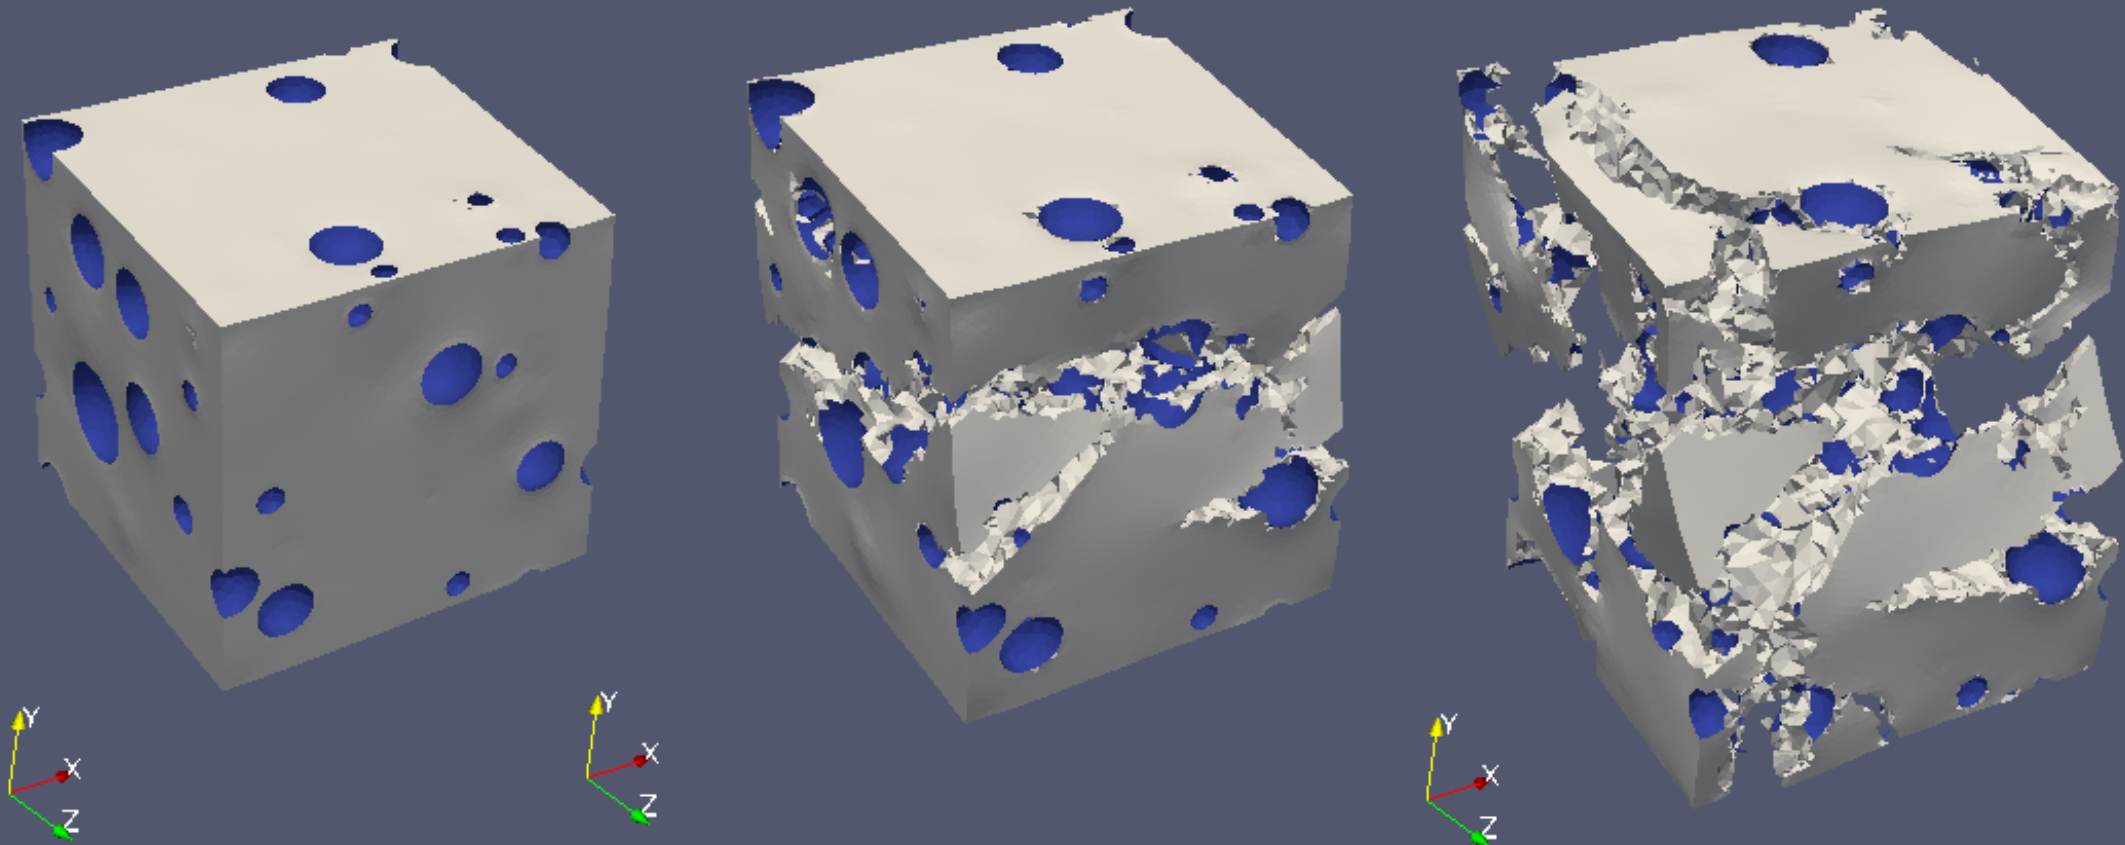
\includegraphics[width=10.cm]{../chapter_000_introduction/figures/VEREsnoul.png}
  \caption{Description of the failure of a representative element volume due to
  the bubble pressurisation in the high burn-up structure
  \cite{esnoul_etude_2018}}
  \label{fig:hho:esnoul}
\end{figure}

Studies at the microstructural scale have emerged in the last decade to
improve the description of the behaviour of the fuel material:

\begin{itemize}
  \item Mixed oxyde fuels have a complex microstructure which depends of the
  manufacturing process. Non-linear homogeneization of those
  microstructures allows deriving the effective macroscopic viscoplastic
  behaviour \cite{el_abdi_generation_2018}. In
  \cite{roussette_analyse_2005, largenton_modelisation_2012, largenton_extension_2019},
  the non-uniform transformation field analysis is used. Based on an
  non-linear extension of \cite{ricaud_effective_2009}, the methodology
  described in \cite{masson_modified_2020} has been used to derive a
  macroscopic viscoplastic behaviour of the MOX fuel.
  \item For uranium dioxide, viscoplasticity has been
  studied at the gain scale in \cite{portelette_crystal_2018} using a
  classical \(\tensor{F}{}_{e}\,\cdot\,\tensor{F}{}_{p}\) approach.
  \item Recent experimental studies have shown that the high burn-up structure
  may lead to a fine-grained fragmentation of the fuel in off-normal
  operating conditions, a phenomena which has been investigated
  numerically in \cite{esnoul_etude_2018} as illustrated in Figure
  \ref{fig:hho:esnoul}; a phenomenon that is expected to be predicted by numerical models of the phase field 
  approach to fracture.
\end{itemize}

% - Mixed oxyde fuels have a complex microstructure which depends of the
%   manufacturing process. Non-linear homogeneization of those
%   microstructures allows deriving the effective macroscopic viscoplastic
%   behaviour \cite{el_abdi_generation_2018}. In
%   \cite{roussette_analyse_2005,largenton_modelisation_2012,@largenton_extension_2019},
%   the non-uniform transformation field analysis is used. Based on an
%   non-linear extension of \cite{ricaud_effective_2009}, the methodology
%   described in \cite{masson_modified_2020} has been used to derive a
%   macroscopic viscoplastic behaviour of the MOX fuel.
% - For uranium dioxide, viscoplasticity has been
%   studied at the gain scale in \cite{portelette_crystal_2018} using a
%   classical \(\tensor{F}{}_{e}\,\cdot\,\tensor{F}{}_{p}\) approach.
% - Recent experimental studies have shown that the high burn-up structure
%   may lead to a fine-grained fragmentation of the fuel in off-normal
%   operating conditions, a phenomena which has been investigated
%   numerically in \cite{esnoul_etude_2018} as illustrated in Figure
%   @fig:hho:esnoul; a phenomenon that is expected to be predicted by numerical models of the phase field approach to fracture.

\subsection{Current numerical limitations of fuel rod simulations}

The previous sections highlighted the fact that the brittle nature of
uranium dioxide and its viscoplastic behaviour at high temperature have
significant roles in the description of the fuel behaviour at the
macroscopic scale. Moreover, we also have highlighted that most
physico-chemical models, which predict the swelling of the fuel, are
coupled with the mechanical resolution by the hydrostatic pressure.

The \texttt{Alcyone} fuel performance code currently uses standard linear
elements to solve the mechanical equilibrium. The reasons for this
choice are mostly twofold:

\begin{itemize}
  \item The contact algorithm of \texttt{Cast3M} is limited to surfaces described by
  linear elements. Contact of quadratic elements can be added by
  linearising the elements (nodes at the middle of edges must follow the
  mean displacement of the corner nodes) with additional Lagrange
  multipliers.
  \item The brittle nature of the fuel is described by a local damage law
  \cite{michel_new_2017} which is regularised by the mesh size to ensure a
  finite fracture energy, following \cite{hillerborg_analysis_1976}. Such
  approach, while efficient, is limited to linear elements to ensure
  that all integration points have the same weights. Moreover, even
  though the dissipated energy is regularised, the crack paths may be
  influenced by the mesh orientation.
\end{itemize}

% - The contact algorithm of \texttt{Cast3M} is limited to surfaces described by
%   linear elements. Contact of quadratic elements can be added by
%   linearising the elements (nodes at the middle of edges must follow the
%   mean displacement of the corner nodes) with additional Lagrange
%   multipliers.
% - The brittle nature of the fuel is described by a local damage law
%   \cite{michel_new_2017} which is regularised by the mesh size to ensure a
%   finite fracture energy, following \cite{hillerborg_analysis_1976}. Such
%   approach, while efficient, is limited to linear elements to ensure
%   that all integration points have the same weights. Moreover, even
%   though the dissipated energy is regularised, the crack paths may be
%   influenced by the mesh orientation.

Linear elements are notably bad at describing materials nearly
incompressible, a caveat called volumetric locking described in Appendix
\ref{sec:hho:volumetric_locking}. Volumetric locking gives rise to spurious
oscillations of the hydrostatic pressure at the integration points.
Those oscillations are all undesirable due to the coupling with the
physico-chemical models.

Challenges associated with crack propagation are twofold:

\begin{itemize}
  \item Handling unstable crack propagation, in particular when simulating the
  initial fragmentation of the pellet described in Section
  \ref{sec:hho:normal_operating_conditions}, is still a major issue
  \cite{michel_new_2017, lu_schema_2019}.
  \item Attempts to use variational approaches to fracture are currently
  limited by the treatment of irreversibility constraints
  \cite{helfer_modelisation_2017, lu_schema_2019}.
\end{itemize}

% - Handling unstable crack propagation, in particular when simulating the
%   initial fragmentation of the pellet described in Section
%   @sec:hho:normal_operating_conditions, is still a major issue
%   \cite{michel_new_2017;@lu_schema_2019}.
% - Attempts to use variational approaches to fracture are currently
%   limited by the treatment of irreversibility constraints
%   \cite{helfer_modelisation_2017;@lu_schema_2019}.
